\documentclass{article}

\usepackage{graphicx} % For including images
\usepackage{amsmath} % For mathematical symbols and equations
\usepackage{booktabs} % For professional-looking tables
\usepackage{hyperref} % For hyperlinks
\usepackage{natbib} % For bibliography management
\usepackage[utf8]{inputenc}
\usepackage{amssymb}
\usepackage{lipsum}
\usepackage{longtable}
\usepackage{subcaption}
\usepackage{changes}

\title{AgriScan: Next.js Powered Cross-Platform Solution for Automated Plant Disease Diagnosis and Crop Health Management}
\date{}

\begin{document}

\maketitle

\begin{abstract}
Plant diseases present a formidable challenge to the agricultural sector worldwide, leading to significant losses, with the United States experiencing annual losses amounting to one-third of crop production. Diagnosis of crop diseases through optical observation of leaf symptoms is particularly daunting for farmers with limited resources. Therefore, there is an urgent need for enhanced detection, monitoring, and prediction methods to mitigate agricultural losses effectively. Harnessing the power of computer vision and Deep Learning (DL), this paper introduces a cross-platform system designed to automate plant leaf disease diagnosis. The system employs Convolutional Neural Networks (CNNs) to classify 46 disease categories, trained on a dataset comprising 96,206 images of healthy and infected plant leaves. The user interface, accessible across multiple platforms including Android, iOS, Windows, and Linux, allows farmers to capture photos of infected leaves and receive real-time disease classification along with confidence percentages. By empowering farmers to maintain crop health and prevent the application of incorrect fertilizers, the system aims to optimize crop productivity. Performance evaluation includes metrics such as classification accuracy and processing time, with the model achieving an impressive overall accuracy of 93.45\% across 46 common disease classes spanning 16 crop species.
\end{abstract}

\section{Introduction}

Plant diseases represent a formidable challenge to global agriculture, exerting significant economic burdens and threatening food security. With the United States alone experiencing annual losses amounting to one-third of crop production due to diseases, it is evident that effective disease management strategies are urgently needed. Traditionally, farmers have relied on visual observation of leaf symptoms to diagnose plant diseases, a process often hindered by subjectivity and the expertise required. This approach becomes even more challenging for farmers with limited resources or access to agricultural experts.

In recent years, advancements in technology, particularly in the fields of computer vision and Deep Learning (DL), have presented new opportunities for revolutionizing disease diagnosis in agriculture. \replaced{CNN's}{Convolutional Neural Networks (CNNs)}, a class of DL algorithms, have demonstrated remarkable capabilities in image recognition tasks, making them well-suited for automated plant disease diagnosis. By leveraging large datasets of labeled images, CNNs can learn to accurately classify diseased plant leaves from healthy ones based on visual patterns and symptoms.

Motivated by the need for more efficient disease management strategies, this paper introduces a novel cross-platform system designed to automate the diagnosis of plant leaf diseases. The system harnesses the power of CNNs to classify 46 disease categories, covering a wide range of common plant diseases affecting 16 different crop species. The development of this system is driven by the recognition that timely and accurate diagnosis is essential for implementing effective disease control measures, thereby minimizing crop losses and optimizing productivity.

In addition to its classification capabilities, the system features a user-friendly interface accessible across multiple platforms, including Android, iOS, Windows, and Linux. This accessibility ensures that farmers, regardless of their technological proficiency or the devices they own, can easily utilize the system to diagnose plant diseases in real-time. By empowering farmers to make informed decisions about disease management practices, the system aims to enhance crop health and reduce reliance on costly and potentially harmful interventions such as excessive pesticide use.

To evaluate the performance of the system, comprehensive metrics such as classification accuracy and processing time are employed. The results demonstrate the system's effectiveness in accurately identifying plant diseases, with an impressive overall accuracy of 93.45% across the 46 disease classes. Furthermore, the system's ability to provide real-time diagnosis enables farmers to take prompt action, thereby minimizing the spread of diseases and mitigating crop losses.

This paper provides a detailed overview of the development, implementation, and evaluation of the proposed system, highlighting its potential to revolutionize plant disease management in agriculture. By integrating advanced technology into traditional farming practices, this system represents a significant step towards sustainable and efficient disease control strategies, ultimately contributing to global food security and agricultural sustainability.



\section{Literature Review}
Recent advancements in the application of machine learning techniques within the agriculture sector have garnered considerable attention from academia [2,3,5,6], industries [1,7], and governmental bodies [8,9]. This section provides an overview of existing research endeavors focusing on the detection of crop diseases employing various machine learning methodologies.

Given the substantial economic losses incurred globally due to plant diseases, significant efforts have been directed towards enhancing crop monitoring and disease diagnosis processes. For instance, in [10], researchers introduced a deep learning model aimed at identifying foliar disease symptoms in cassava plants. They utilized a convolutional neural network (CNN) trained on a dataset comprising 720 diseased leaf samples collected from agricultural fields in Tanzania. This model successfully categorized seven classes of cassava leaflets, including healthy ones and those afflicted with diseases such as brown streak disease, mosaic disease, green mite damage, red mite damage, brown leaf spot, and nutrient deficiency. However, its practical applicability for detecting cassava diseases in real-world images was limited by a low classification rate.

Chen et al. [6] employed a fusion of Internet of Things (IoT) and Artificial Intelligence (AI) technologies to detect early stages of rice blast disease. They developed an IoT platform named RiceTalk, which utilized non-image IoT devices to collect sensing data from soil cultivation. This data was then processed in real-time by a CNN model, achieving an average prediction accuracy of 89.4\% for detecting rice blast disease in natural agricultural settings.

Another noteworthy development is presented in [2], where a deep learning-based platform for detecting crop diseases and insect pests was proposed. Similar to [6], CNN served as the underlying deep learning engine to identify 27 crop diseases prevalent in the challenging mountainous terrain of China. The system was designed with a user-friendly Java applet interface, facilitating convenient usage by Chinese farmers. Experimental results demonstrated an overall recognition accuracy of 86.1%.

Jiang et al. [5] proposed an approach for detecting apple leaf diseases based on the Mask Region-based CNN (R-CNN) model. R-CNN, known for object instance segmentation, was employed to detect various apple diseases using a dataset comprising 2029 images of diseased apple leaves. Despite the relatively small dataset used for training, the developed model achieved a classification accuracy of 78.8%.

In [3], researchers introduced a deep learning-based method for assessing the severity of citrus diseases. They trained six deep learning models, including AlexNet, DenseNet-169, Inception-v3, ResNet-34, SqueezeNet-1.1, and VGG13, on a dataset containing 5406 images of infected citrus leaves. Data augmentation techniques were employed to enhance the models' learning performance, resulting in the highest classification accuracy of 92.60% achieved by the Inception-v3 model.

Additionally, the potential of hyperspectral imaging for plant disease detection and protection was explored in [4]. The authors discussed fundamental principles of hyperspectral measurements and highlighted the influence of factors such as camera spatial resolution and the number of mixed pixels on the information content of hyperspectral images.

In summary, the reviewed literature on plant disease detection utilizing machine learning and computer vision approaches underscores the focus on specific disease classes [5,10], crop varieties [3], geographical regions [2,10], or countries. Moreover, while most deep learning-based models operate offline, their deployment on mobile devices remains impractical due to computational constraints, limiting their real-time applicability and hindering the user experience in agricultural settings.

\section{Training Methodology}

\subsection{Dataset Selection}

The dataset[11] employed in this project comprises images of various plant leaves afflicted by various diseases, with a sample image depicted in Fig. 1. These images were sourced from the extensive Plant Diseases Training Dataset, housing a repository of more than 95,000 images spanning 16 diverse crops, encompassing Apple, Bell Paper, Blueberry, Cassava, Cherry, Corn Grape, Orange, Peach, Potato, Raspberry, Rice, Soybeans, Squash, Strwaberry, Suger-cane and Tomato. For this project, all image classes were utilized.

\begin{figure}[h]
    \centering
    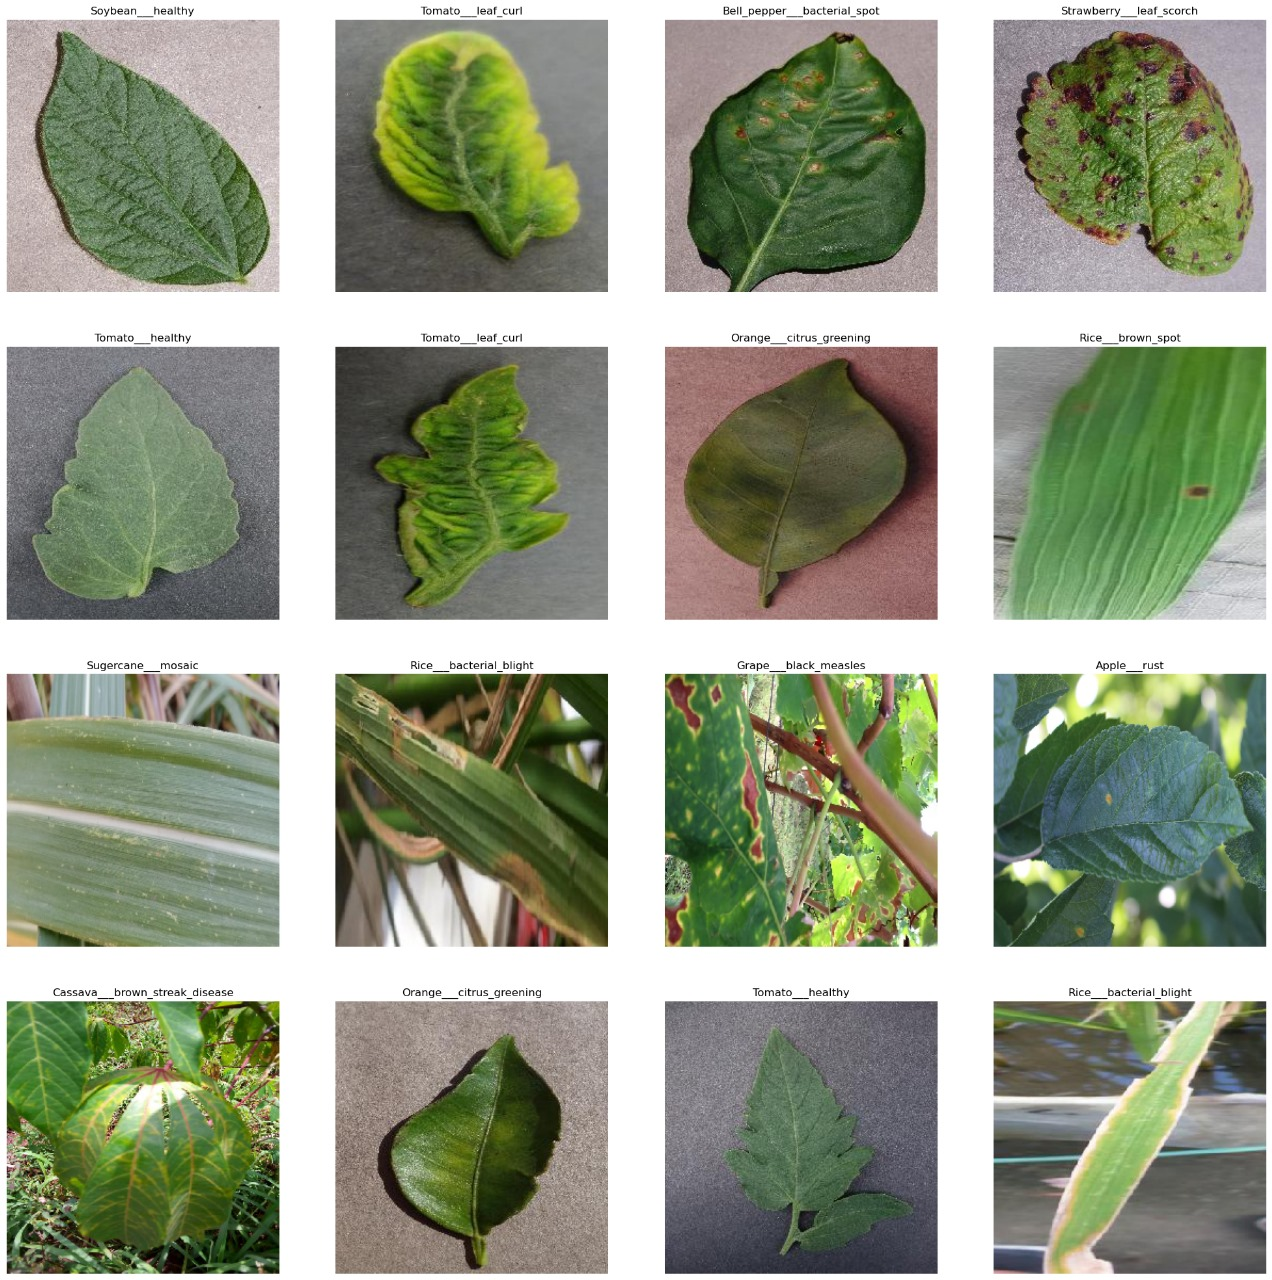
\includegraphics[width=0.90\textwidth]{sample_image.jpg}
    \caption{Sample of image data.}
    \label{fig:sample_image}
\end{figure}

The dataset comprises 46 distinct disease types and their healthy counterpart having a total of 61 class., including Apple alternaria leaf spot, Apple black rot, Apple brown spot, Apple gray spot, Apple rust, Apple scab, Bell pepper bacterial spot, Cassava bacterial blight, Cassava brown streak disease, Cassava green mottle, Cassava mosaic disease, Cherry powdery mildew, Corn common rust, Corn gray leaf spot, Corn northern leaf blight, Grape black measles, Grape black rot, Grape isariopsis leaf spot, Grape leaf blight, Orange citrus greening, Peach bacterial spot, Potato bacterial wilt, Potato early blight, Potato late blight, Potato nematode, Potato pests, Potato phytophthora, Potato virus, Rice bacterial blight, Rice blast, Rice brown spot, Rice tungro, Squash powdery mildew, Sugarcane mosaic, Sugarcane red rot, Sugarcane rust, Sugarcane yellow leaf, Tomato bacterial spot, Tomato early blight, Tomato late blight, Tomato leaf curl, Tomato leaf mold, Tomato mosaic virus, Tomato septoria leaf spot, and Tomato spider mites. The training dataset comprised 95,400 images, with each class having varying amounts of image data available, ranging from a few hundred to several thousand, as illustrated in Figure \ref{fig:image_amount}. Examples of sample images are provided in Figure \ref{fig:sample_image}.

\begin{figure}[h]
  \centering
  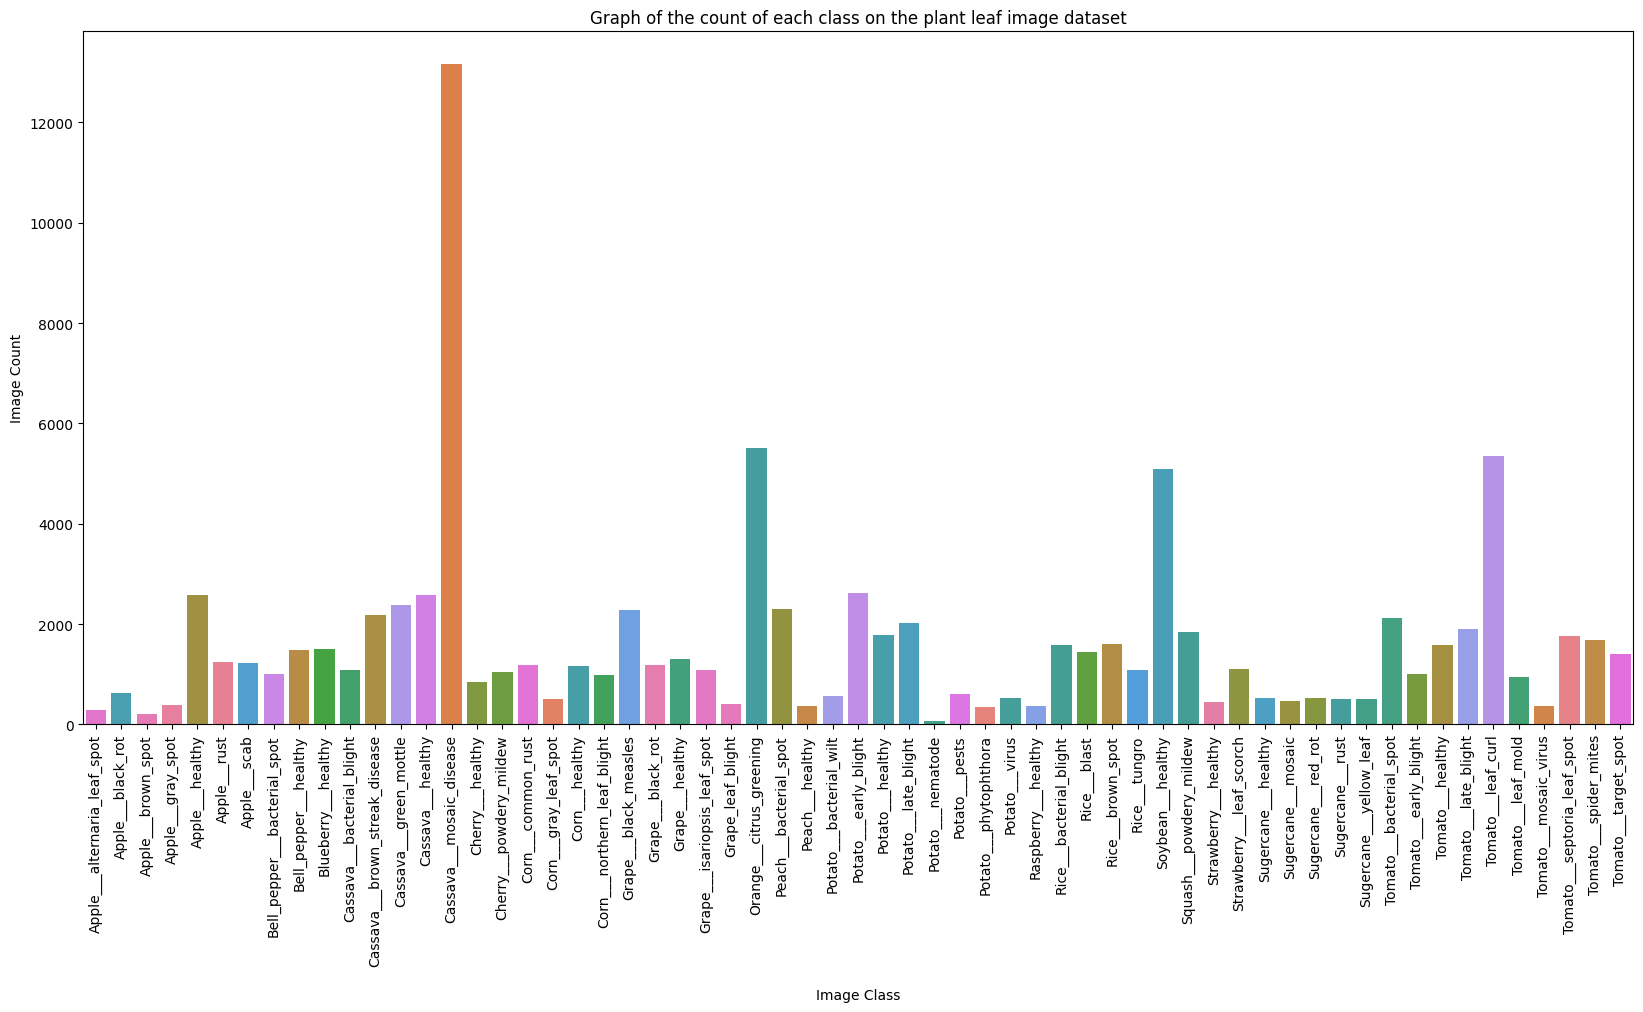
\includegraphics[width=1.0\textwidth]{image_amount}
  \caption{Plot of data count of each class in the dataset.}
  \label{fig:image_amount}
\end{figure}

\subsection{Model Selection}
The model selected for our application is LDDTA[12], as detailed in the journal titled "Comparing pre-trained models for efficient leaf disease detection: a study on custom CNN." Within this research, the team undertook a comprehensive comparison of ten widely recognized pre-trained Convolutional Neural Networks alongside their own bespoke design, LDDTA.

This investigation involved an in-depth analysis of various pre-trained models to assess their efficacy in leaf disease detection tasks. In addition to these established models, the researchers developed LDDTA from scratch, tailoring it specifically for this domain.

The study aimed to evaluate the performance of these models across a range of metrics, including accuracy, computational efficiency, and robustness in handling diverse datasets. By subjecting both pre-trained models and the custom-built LDDTA to rigorous testing and comparative analysis, the researchers sought to provide valuable insights into the most suitable architectures for efficient leaf disease detection.

Through meticulous experimentation and thorough evaluation, the study shed light on the strengths and limitations of each model, offering valuable guidance for researchers and practitioners in the field of agricultural image analysis.

\subsection{Model Architecture}

In their study[12], researchers intricately crafted a \replaced{CNN}{Convolutional Neural Network (CNN)} model, as depicted in Figure \ref{fig:lddta}, specifically tailored for image classification tasks, pivotal in the realm of computer vision. Leveraging the Keras API, they seamlessly assembled deep neural networks layer by layer.

They initiated the process by applying preprocessing steps to resize and rescale input images, ensuring uniformity and proper scaling before feeding them into the network. Subsequently, a series of convolutional layers were incorporated to extract hierarchical features from the images.

The first convolutional layer comprised 32 filters, each sized $3 \times 3$, adept at recognizing intricate patterns within the images. The researchers applied the rectified linear unit (ReLU) activation function to introduce nonlinearity, capturing complex relationships in the data.

Interspersed between the convolutional layers were max pooling layers, aimed at reducing spatial dimensions while retaining salient features. Max pooling with a pool size of $2 \times 2$ was employed, effectively down-sampling the feature maps.

\begin{figure}[h]
    \centering
    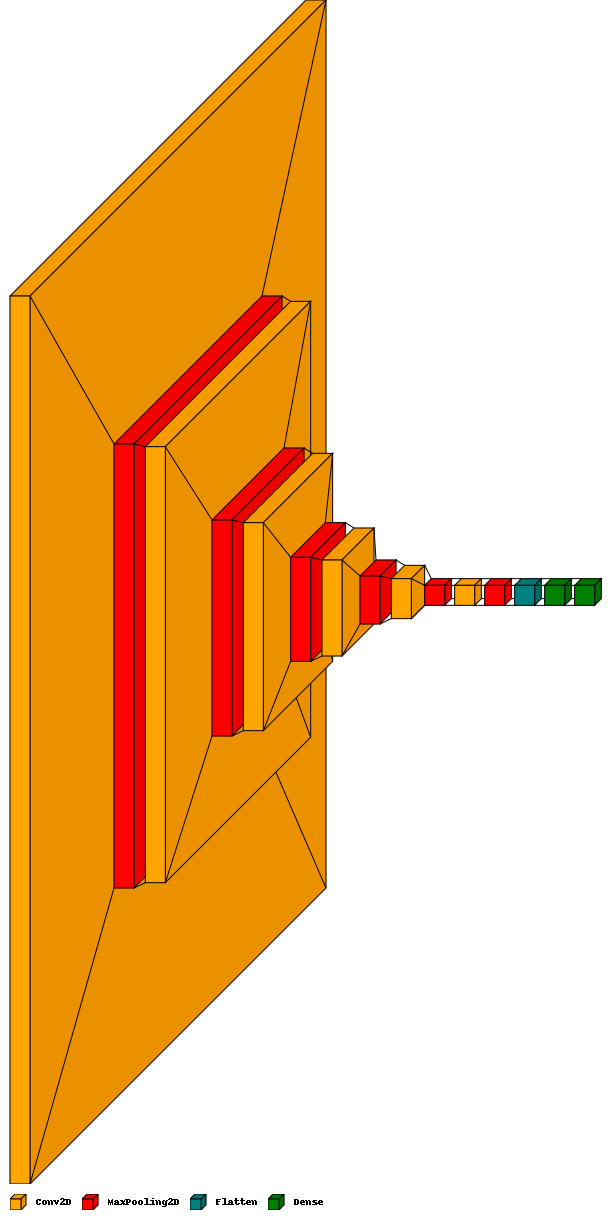
\includegraphics[width=0.60\textwidth, height=0.4\textheight]{lddta_architecture}
    \caption{Architecture of the Proposed Leaf Disease Detection Model \deleted{(LDDTA)}.}
    \label{fig:lddta}
\end{figure}

As the network deepened, the complexity of learned features was augmented by doubling the number of filters in each subsequent convolutional layer, allowing the model to extract increasingly intricate representations from the images. The layers were systematically organized with a sequence of convolution followed by max pooling for efficient feature extraction and dimensionality reduction.

After extracting hierarchical features, a flattening operation was performed to transform the multi-dimensional tensor into a linear vector, preparing the data for fully connected layers.

The first fully connected layer consisted of 64 neurons, each activated by the ReLU function. This dense layer facilitated high-level feature aggregation and abstraction, enabling the model to grasp abstract concepts present in the images.

Finally, the output layer, comprising as many neurons as there were distinct classes in the classification task, employed the softmax activation function. This activation computed class probabilities, enabling the model to make informed and confident predictions.


\subsection{Dataset Preprocessing}
To construct the training dataset, 500 images were randomly sampled from each class in the training set and relocated from their respective folders. The remaining images in the training dataset were then utilized to generate similar images using the Augmenter package in Python. This approach encompasses techniques such as rotation, flipping, cropping, and resizing of existing images to produce new ones. The objective was to ensure that each class in the training dataset comprised an equal number of images (500), thus averting bias towards any specific class during the training phase of the \replaced{CNN}{Convolutional Neural Network (CNN)} and the pre-trained neural networks.

In cases where the number of images in a particular class was less than 500, data augmentation techniques were employed to generate additional images. Conversely, if the number of images in a class surpassed 500, only the initial 500 images were retained.

Subsequently, the images were categorized into three groups: training, testing, and validation, with 83.5\% allocated for training, 8.3\% for testing, and 8.3\% for validation.

All images in the dataset were in JPEG format and exhibited varying resolutions. Hence, they were standardized to a size of 256x256 pixels. The utilization of a diverse and meticulously curated dataset, such as the Plant Diseases Training Dataset, coupled with appropriate data preprocessing techniques, is imperative for the development of an accurate and reliable machine learning model for disease detection in plant leaves.


\subsection{Dataset Augmentation}
To expand the diversity of the training dataset, data augmentation techniques were applied. This involved manipulating existing images through operations such as rotation, flipping, cropping, and resizing using the Augmenter package in Python. The goal was to generate new images that exhibit variations while preserving the essential features relevant for disease detection. Some example aumneted examples are shown in figure \ref{fig:augmented_image}.

In cases where a class had fewer than 500 images, augmentation techniques were employed to generate additional samples. Conversely, for classes with over 500 images, only the first 500 were utilized to maintain balance within the dataset.

\begin{figure}[h]
    \centering
    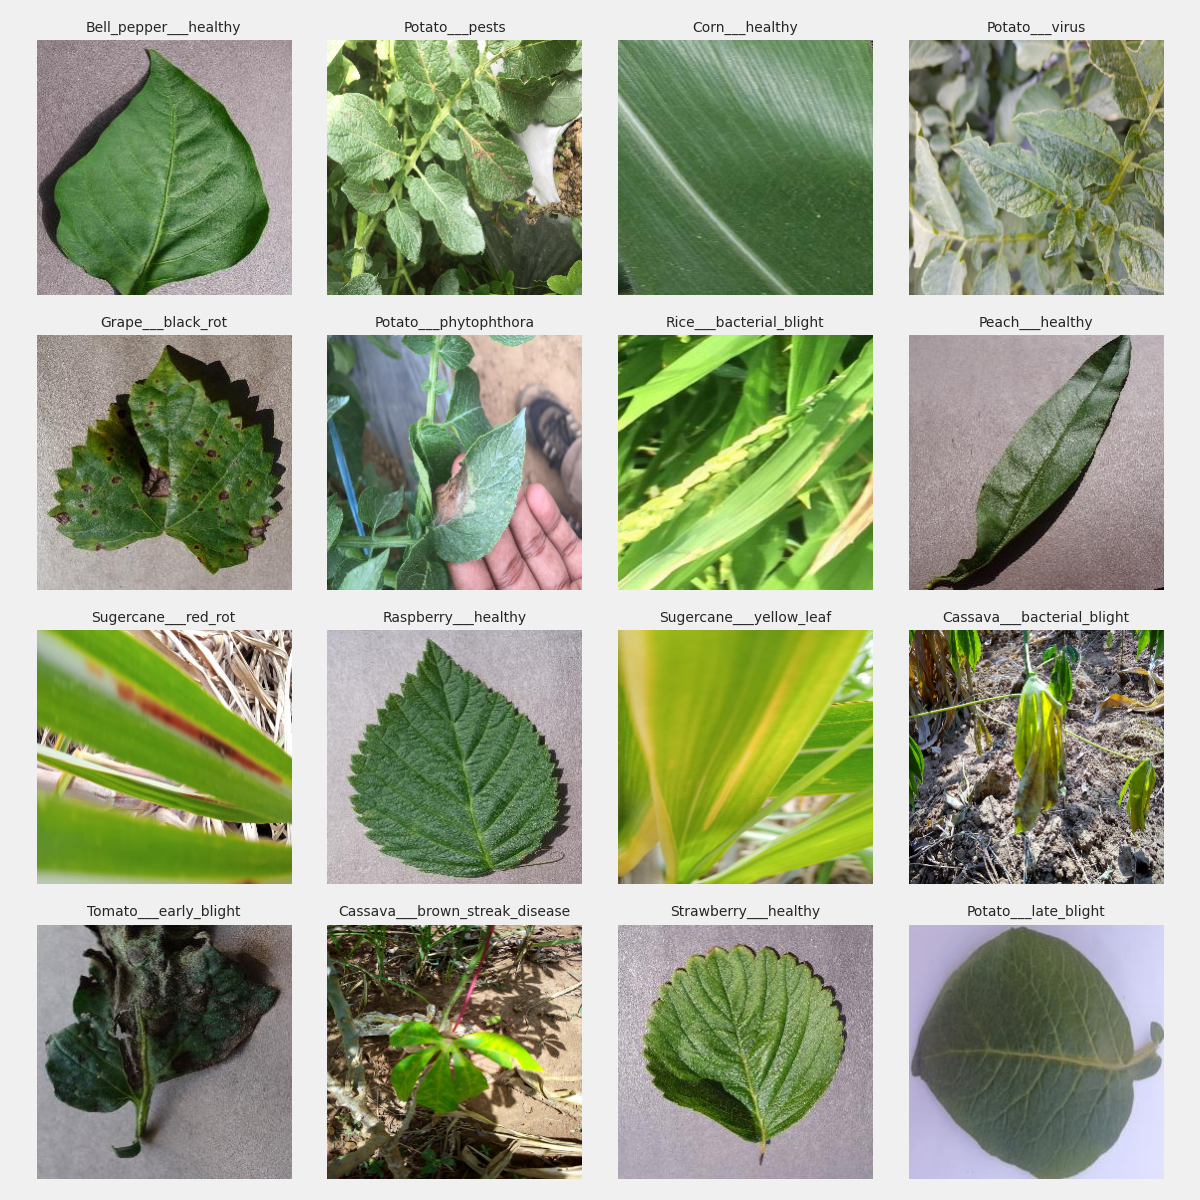
\includegraphics[width=1.00\textwidth]{augmented_images_plot.png}
    \caption{Sample of augmented image data.}
    \label{fig:augmented_image}
\end{figure}

\section{Dataset Preparation}
To ensure uniformity and compatibility, all images in the dataset were standardized to a resolution of 256x256 pixels. The dataset was then divided into three subsets: training, testing, and validation as shown in figure \ref{fig:data_distribution}. 83.5\% of the images were allocated for training, 8.3\% for testing, and 8.3\% for validation.

\begin{figure}[h]
    \centering
    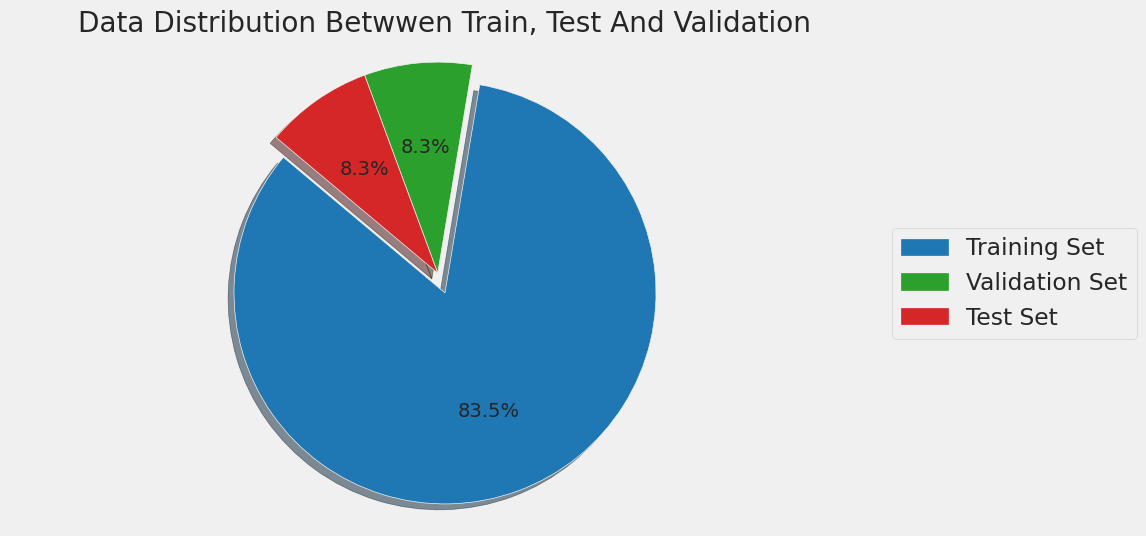
\includegraphics[width=1.00\textwidth]{data_distribution.png}
    \caption{Data distribution Pie-chart.}
    \label{fig:data_distribution}
\end{figure}

The utilization of a diverse and meticulously curated dataset, such as the Plant Diseases Training Dataset, coupled with appropriate data preprocessing techniques, is imperative for the development of an accurate and reliable machine learning model for disease detection in plant leaves.



\subsection{Model Architecture}
\textbf{Input Layer (Resize and Rescale):}

This layer resizes and rescales the input images to a standard size suitable for processing by the neural network.

\textbf{Convolutional Layer 1:}
\begin{itemize}
    \item Number of filters: 32
    \item Kernel size: $(3, 3)$
    \item Activation function: ReLU (Rectified Linear Unit)
    \item Input shape: Defined by \texttt{input\_shape}
\end{itemize}

The first convolutional layer applies 32 filters of size $3 \times 3$ to the input image. Each filter extracts specific features, such as edges or textures, from different parts of the image. The ReLU activation function introduces non-linearity to the model, allowing it to learn complex patterns.

\textbf{Max Pooling Layer 1:}
\begin{itemize}
    \item Pool size: $(2, 2)$
\end{itemize}

The max-pooling layer reduces the spatial dimensions of the feature maps produced by the previous convolutional layer. It does this by retaining only the maximum value in each $2 \times 2$ region, effectively downsampling the feature maps.

\textbf{Convolutional Layer 2:}
\begin{itemize}
    \item Number of filters: 64
    \item Kernel size: $(3, 3)$
    \item Activation function: ReLU
\end{itemize}

Subsequent convolutional layers further extract increasingly abstract features from the input. In this layer, 64 filters are applied to the feature maps generated by the previous layer.

\textbf{Max Pooling Layer 2:}
\begin{itemize}
    \item Pool size: $(2, 2)$
\end{itemize}

Similar to the first max-pooling layer, this layer further reduces the spatial dimensions of the feature maps.

% Repeat similar explanations for the remaining layers...

\textbf{Flatten Layer:}
Flattens the input from the previous layer into a one-dimensional vector. This is necessary to feed the data into the fully connected layers.

\textbf{Dense Layer 1:}
\begin{itemize}
    \item Number of neurons: 64
    \item Activation function: ReLU
\end{itemize}

The fully connected layers process the flattened features and perform high-level reasoning. This layer consists of 64 neurons with ReLU activation.

\textbf{Output Layer (Dense Layer 2):}
\begin{itemize}
    \item Number of neurons: $n\_classes$
    \item Activation function: Softmax
\end{itemize}

The final layer produces the output predictions. It consists of $n\_classes$ neurons, each representing the probability of the input belonging to a particular class. The softmax activation function ensures that the output probabilities sum up to 1, making it suitable for multi-class classification tasks.

This model architecture effectively learns hierarchical representations of the input data, starting from low-level features in the early layers to more abstract features in the deeper layers, ultimately enabling accurate classification.



\subsection{Training and Validation Loss Analysis}
The authors originally intended to train the proposed model for 50 epochs. However, due to early stopping criteria, the training concluded at the 14th epoch. The performance metrics, including training and validation accuracies, are illustrated in Figure \ref{fig:training_plot_loss_acc}. The loss computation during training and validation phases was conducted using categorical cross-entropy, as defined by the following equation:

\begin{equation}
\text{Loss} = -\frac{1}{M} \sum_{c=1}^{M} y_c \log(p_c)
\end{equation}

Here, $M$ denotes the number of classes, $y_c$ represents a binary indicator (0 or 1) indicating whether class label $c$ is the correct classification for observation $o$, and $p_c$ is the predicted probability that observation $o$ belongs to class $c$. Subsequent to analyzing the model's performance, the authors proceeded with testing, employing a dataset comprising 1207 samples.

\begin{figure}[h]
    \centering
    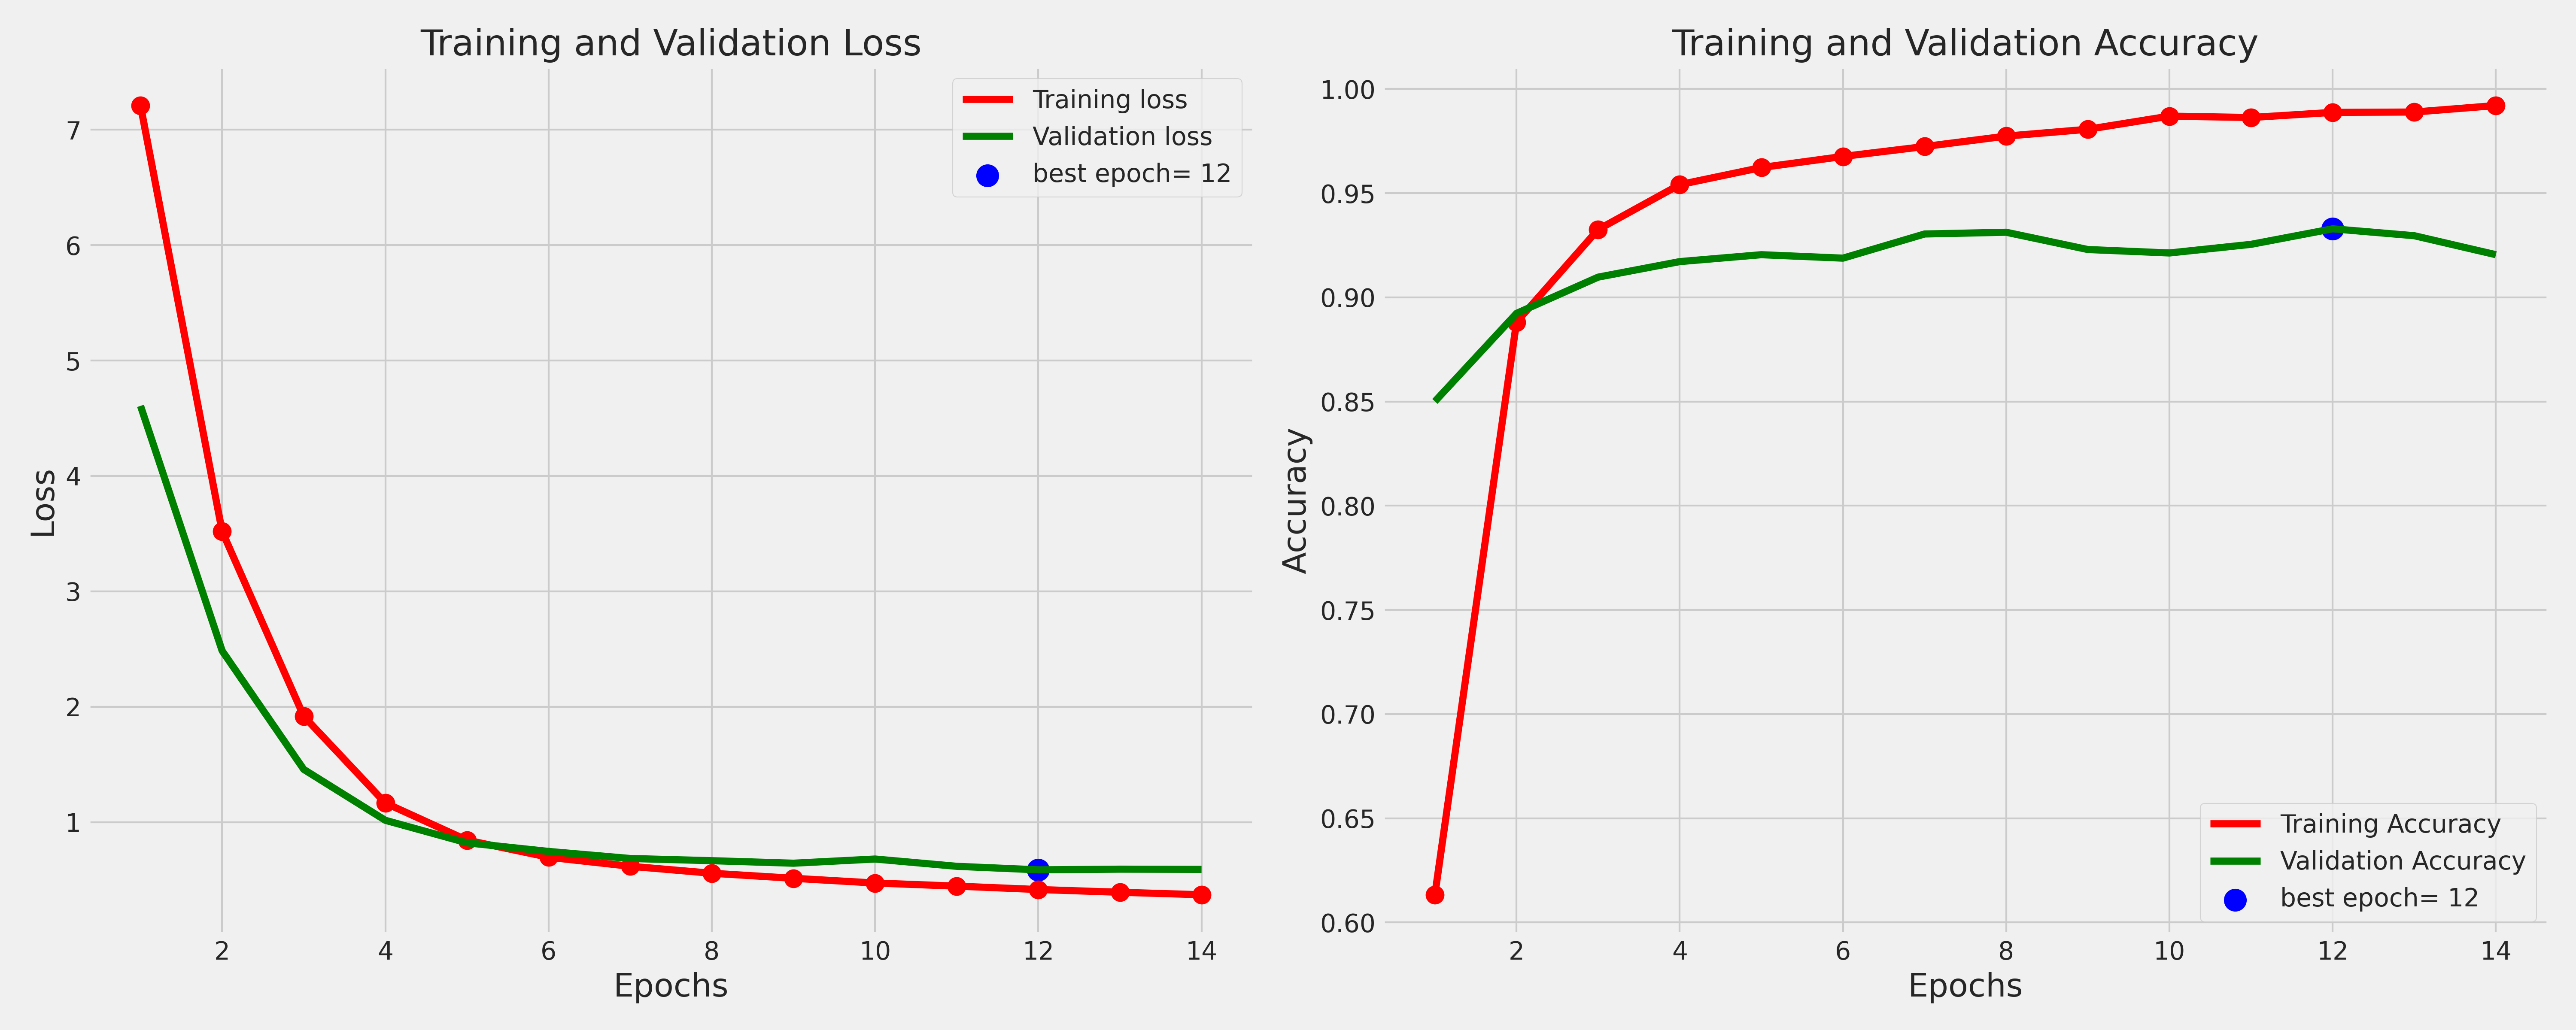
\includegraphics[width=1.00\textwidth]{training_plot_loss_acc.png}
    \caption{Plot of Training and Validation Accuracy and Loss curve.}
    \label{fig:training_plot_loss_acc}
\end{figure}

In Figure \ref{fig:training_plot_loss_acc}, the training loss and validation loss curves of the proposed model are depicted. These curves offer valuable insights into the model's behavior during training. The training loss delineates the disparity between the predicted values and the actual target values within the training dataset. Over the course of training, the ideal scenario is a gradual decrease in training loss, indicative of the model's enhanced ability to fit the training data.

Conversely, the validation loss assesses the model's generalization performance on unseen data. It is computed using a separate validation dataset that the model has not encountered during training. Similar to the training loss, the validation loss ideally diminishes initially, reflecting the model's improved capability to generalize its learnings to new instances.



\subsubsection{Performance Metrics}

The table \ref{tab:perfromance_metrics} presents the performance metrics of a classification model evaluated on a dataset containing various classes of plant diseases. Precision, recall, F1-score, and support are reported for each class, along with macro and weighted averages across all classes.

Precision measures the accuracy of positive predictions, recall measures the ability of the model to find all the relevant cases within the dataset, and F1-score provides a balance between precision and recall. Support refers to the number of actual occurrences of the class in the specified dataset.

The classification model achieved an accuracy of 93.45\%. The macro-average F1-score, which considers the unweighted mean of F1-scores for each class, is 93.38\%. The weighted average F1-score, which considers the F1-scores for each class weighted by the number of samples in each class, is 93.31\%.


\begin{center}
\begin{longtable}{lcccc}
\hline
\textbf{Class} & \textbf{Precision} & \textbf{Recall} & \textbf{F1-Score} & \textbf{Support} \\
\hline
\endhead
Apple\_alternaria\_leaf\_spot & 1.0000 & 1.0000 & 1.0000 & 20 \\
Apple\_black\_rot & 1.0000 & 1.0000 & 1.0000 & 20 \\
Apple\_brown\_spot & 0.9524 & 1.0000 & 0.9756 & 20 \\
Apple\_gray\_spot & 0.9500 & 0.9500 & 0.9500 & 20 \\
Apple\_healthy & 1.0000 & 0.9500 & 0.9744 & 20 \\
Apple\_rust & 1.0000 & 0.9500 & 0.9744 & 20 \\
Apple\_scab & 1.0000 & 0.9500 & 0.9744 & 20 \\
Bell\_pepper\_bacterial\_spot & 1.0000 & 1.0000 & 1.0000 & 20 \\
Bell\_pepper\_healthy & 1.0000 & 1.0000 & 1.0000 & 20 \\
Blueberry\_healthy & 1.0000 & 1.0000 & 1.0000 & 20 \\
Cassava\_bacterial\_blight & 0.8000 & 0.8000 & 0.8000 & 20 \\
Cassava\_brown\_streak\_disease & 0.7222 & 0.6500 & 0.6842 & 20 \\
Cassava\_green\_mottle & 0.6250 & 0.5000 & 0.5556 & 20 \\
Cassava\_healthy & 0.4583 & 0.5500 & 0.5000 & 20 \\
Cassava\_mosaic\_disease & 0.8095 & 0.8500 & 0.8293 & 20 \\
Cherry\_healthy & 1.0000 & 1.0000 & 1.0000 & 20 \\
Cherry\_powdery\_mildew & 1.0000 & 1.0000 & 1.0000 & 20 \\
Corn\_common\_rust & 0.9524 & 1.0000 & 0.9756 & 20 \\
Corn\_gray\_leaf\_spot & 0.9091 & 1.0000 & 0.9524 & 20 \\
Corn\_healthy & 0.9500 & 0.9500 & 0.9500 & 20 \\
Corn\_northern\_leaf\_blight & 1.0000 & 0.9000 & 0.9474 & 20 \\
Grape\_black\_measles & 1.0000 & 1.0000 & 1.0000 & 20 \\
Grape\_black\_rot & 1.0000 & 1.0000 & 1.0000 & 20 \\
Grape\_healthy & 0.9524 & 1.0000 & 0.9756 & 20 \\
Grape\_isariopsis\_leaf\_spot & 0.3333 & 0.1500 & 0.2069 & 20 \\
Grape\_leaf\_blight & 0.4516 & 0.7000 & 0.5490 & 20 \\
Orange\_citrus\_greening & 1.0000 & 1.0000 & 1.0000 & 20 \\
Peach\_bacterial\_spot & 1.0000 & 1.0000 & 1.0000 & 20 \\
Peach\_healthy & 0.9524 & 1.0000 & 0.9756 & 20 \\
Potato\_bacterial\_wilt & 1.0000 & 1.0000 & 1.0000 & 20 \\
Potato\_early\_blight & 1.0000 & 1.0000 & 1.0000 & 20 \\
Potato\_healthy & 1.0000 & 0.9500 & 0.9744 & 20 \\
Potato\_late\_blight & 1.0000 & 1.0000 & 1.0000 & 20 \\
Potato\_nematode & 1.0000 & 1.0000 & 1.0000 & 7 \\
Potato\_pests & 1.0000 & 0.9500 & 0.9744 & 20 \\
Potato\_phytophthora & 0.8696 & 1.0000 & 0.9302 & 20 \\
Potato\_virus & 0.9524 & 1.0000 & 0.9756 & 20 \\
Raspberry\_healthy & 1.0000 & 1.0000 & 1.0000 & 20 \\
Rice\_bacterial\_blight & 0.9524 & 1.0000 & 0.9756 & 20 \\
Rice\_blast & 0.9524 & 1.0000 & 0.9756 & 20 \\
Rice\_brown\_spot & 1.0000 & 0.9000 & 0.9474 & 20 \\
Rice\_tungro & 1.0000 & 1.0000 & 1.0000 & 20 \\
Soybean\_healthy & 1.0000 & 1.0000 & 1.0000 & 20 \\
Squash\_powdery\_mildew & 1.0000 & 1.0000 & 1.0000 & 20 \\
Strawberry\_healthy & 1.0000 & 1.0000 & 1.0000 & 20 \\
Strawberry\_leaf\_scorch & 1.0000 & 1.0000 & 1.0000 & 20 \\
Sugercane\_healthy & 0.7600 & 0.9500 & 0.8444 & 20 \\
Sugercane\_mosaic & 1.0000 & 0.8500 & 0.9189 & 20 \\
Sugercane\_red\_rot & 1.0000 & 0.9500 & 0.9744 & 20 \\
Sugercane\_rust & 1.0000 & 0.9500 & 0.9744 & 20 \\
Sugercane\_yellow\_leaf & 0.9500 & 0.9500 & 0.9500 & 20 \\
Tomato\_bacterial\_spot & 0.9091 & 1.0000 & 0.9524 & 20 \\
Tomato\_early\_blight & 0.9500 & 0.9500 & 0.9500 & 20 \\
Tomato\_healthy & 1.0000 & 1.0000 & 1.0000 & 20 \\
Tomato\_late\_blight & 1.0000 & 0.8500 & 0.9189 & 20 \\
Tomato\_leaf\_curl & 1.0000 & 1.0000 & 1.0000 & 20 \\
Tomato\_leaf\_mold & 1.0000 & 1.0000 & 1.0000 & 20 \\
Tomato\_mosaic\_virus & 1.0000 & 1.0000 & 1.0000 & 20 \\
Tomato\_septoria\_leaf\_spot & 1.0000 & 0.9500 & 0.9744 & 20 \\
Tomato\_spider\_mites & 1.0000 & 1.0000 & 1.0000 & 20 \\
Tomato\_target\_spot & 1.0000 & 1.0000 & 1.0000 & 20 \\
\hline
\textbf{Accuracy} & & & 0.9345 & 1207 \\
\textbf{Macro Avg} & 0.9363 & 0.9352 & 0.9338 & 1207 \\
\textbf{Weighted Avg} & 0.9356 & 0.9345 & 0.9331 & 1207 \\
\hline
\caption{Performance Metrics}
\label{tab:perfromance_metrics}
\end{longtable}
\end{center}

\subsubsection{Cross-Validation}
The model's performance was evaluated using cross-validation with the \textit{k}-fold method, where \textit{k} was set to 5. The average performance metrics across all folds are summarized below:

\begin{table}[!htb]
\centering
\begin{tabular}{@{}lcccc@{}}
\toprule
\textbf{Metric}         & \textbf{Precision} & \textbf{Recall} & \textbf{F1-Score} & \textbf{Accuracy (\%)} \\ \midrule
Macro Average           & 93.63\%              & 93.52\%           & 93.38\%              & 93.63\%                    \\
Weighted Average        & 93.56\%              & 93.45\%           & 93.31\%              & 93.45\%                    \\ \bottomrule
\end{tabular}
\caption{Average Performance Metrics}
\label{tab:cross-validation}
\end{table}


The table \ref{tab:cross-validation} shows the macro-average precision, recall, and F1-score were 93.63\%, 93.52\%, and 93.38\%, respectively. The weighted average precision, recall, and F1-score were 93.56\%, 93.45\%, and 93.31\%, respectively.



\section{App Development Methodology}

\subsection{User Interface Design}

In designing the user interface (UI) for the plant leaf disease detection app, several considerations were taken into account. Firstly, the UI should be intuitive and easy to navigate, allowing users to easily upload images of plant leaves for analysis. Additionally, clear feedback should be provided to users during the image processing and disease detection stages to keep them informed of the app's progress.

\subsubsection{UI/UX Considerations}

The user experience (UX) of the app is crucial for its success. It's essential to create a seamless flow from uploading images to viewing the results of the disease detection. This includes optimizing image uploading speeds, providing informative notifications, and ensuring that the UI design is visually appealing and accessible across different devices and screen sizes.


\subsection{Choosing a Framework for Frontend}

Next.js is chosen as the frontend framework for several reasons. Firstly, Next.js offers server-side rendering (SSR) and static site generation (SSG) out of the box, which can significantly improve the app's performance by pre-rendering pages and serving them as static HTML files or rendering them on the server dynamically. This is particularly advantageous for SEO and initial page load times, which are crucial for user experience.

Secondly, Next.js provides built-in support for TypeScript, which enhances code quality and maintainability by adding static typing to JavaScript code. This helps catch errors early in the development process and provides better tooling support for developers.

Additionally, Next.js seamlessly integrates with Tailwind CSS, a utility-first CSS framework, which offers a more efficient and consistent way to style components compared to raw CSS or styled-components. Tailwind CSS provides a wide range of pre-built utility classes that can be used to style components directly in the HTML markup, reducing the need for writing custom CSS code and improving developer productivity.

Furthermore, Next.js offers a streamlined development experience with features like hot module replacement (HMR), automatic code splitting, and built-in support for Tailwind CSS. These features help speed up development time and make it easier to manage dependencies and styling in the frontend codebase.




\subsection{Choosing a Framework for Backend}

Flask is selected as the backend framework for several compelling reasons. Firstly, Flask is lightweight and minimalist, providing just the essentials for building web applications without imposing unnecessary overhead. This simplicity makes Flask well-suited for our project, as it allows us to focus on implementing the specific functionality required for plant leaf disease detection without being encumbered by unnecessary complexity.

Secondly, Flask offers excellent flexibility and extensibility, allowing developers to easily integrate additional libraries and extensions as needed for our project's requirements. Whether it's integrating with machine learning libraries for image processing, connecting to databases for data storage, or implementing authentication and authorization mechanisms, Flask provides a robust foundation upon which we can build and extend our application's functionality.

Additionally, Flask's RESTful request handling capabilities make it well-suited for developing the backend API required for our app. Flask allows us to define routes and endpoints that map HTTP requests to specific functions, enabling us to implement the necessary functionality for image uploading, processing, and result retrieval in a clear and organized manner.

Furthermore, Flask's active and supportive community provides access to a wealth of resources, tutorials, and extensions that can aid in the development process and help address any challenges or obstacles encountered along the way. This community-driven ecosystem ensures that we have access to the tools and support needed to build and maintain a successful backend for our plant leaf disease detection app.



\subsection{Developing the Backend (Flask)}

With Flask selected as the backend framework, we'll proceed with developing the backend functionality required for our plant leaf disease detection app. This involves implementing routes, request handlers, and data processing logic to handle image uploads, run disease detection algorithms, and serve analysis results to the frontend.

We'll start by setting up the Flask application and defining the necessary routes to handle different API endpoints. We'll create routes for uploading images, retrieving analysis results, and possibly handling user authentication and registration if required.

Once the routes are defined, we'll implement the corresponding request handlers to process incoming requests and perform the required actions. This will involve validating input data, running image processing algorithms for disease detection, and generating analysis reports bdased on the results.

To handle image uploads, we'll utilize Flask's file upload capabilities, ensuring that uploaded images are securely stored and processed on the server.

For running disease detection algorithms, we'll integrate the libraries TensorFlow. This library will enable us to analyze uploaded images and identify any signs of plant leaf diseases accurately.

Once the analysis is complete, we'll format the results JSON and return them to the frontend for display. We'll also implement error handling and appropriate HTTP status codes to provide informative responses to the frontend in case of any issues or errors during the processing.

Throughout the development process, we'll adhere to best practices for Flask development, including proper error handling, data validation, and security measures to ensure the reliability and security of our backend API. We'll also thoroughly test the backend functionality using unit tests and integration tests to verify its correctness and robustness before deploying it to production.

By following these steps, we'll develop a robust and scalable backend for our plant leaf disease detection app, leveraging Flask's flexibility and simplicity to deliver a reliable and efficient solution for our users.



\subsubsection{API Design}

The API design for our plant leaf disease detection app revolves around a single endpoint: \texttt{/predict}. This endpoint will handle the prediction of plant leaf diseases based on uploaded images and return the results to the frontend for display.

\textbf{Endpoint:} \texttt{/predict}

\textbf{HTTP Method:} POST

\textbf{Request Body:}
\begin{itemize}
    \item \texttt{image} (file): The image of the plant leaf to be analyzed for disease detection. This will be sent as a multipart/form-data request.
\end{itemize}

\textbf{Response:}
\begin{itemize}
    \item \texttt{status} (string): Indicates the status of the request (e.g., "success" or "error").
    \item \texttt{message} (string): A human-readable message providing additional information about the request status.
    \item \texttt{class} (string): A human-readable message the predicted disease.
    \item \texttt{confidence} (float): A human-readable number providing the confidence percent in float.
\end{itemize}

\textbf{Example Request:}
\begin{verbatim}
POST /predict
Content-Type: multipart/form-data

image: [binary image data]
\end{verbatim}

\textbf{Example Response (Success):}
\begin{verbatim}
{
    "status": "success",
    "message": "Disease detection analysis successful.",
    "class": "Disease\_Name",
    "confidence": float\_value
    
}
\end{verbatim}

\textbf{Example Response (Error):}
\begin{verbatim}
{
    "status": "error",
    "message": "Failed to analyze the provided image."
}
\end{verbatim}

The \texttt{/predict} endpoint follows RESTful principles and accepts POST requests with multipart/form-data containing the image to be analyzed. Upon successful analysis, it returns a JSON response with the status, message, and disease detection results. Error responses provide information about any issues encountered during analysis.



\subsection{Developing the Frontend (Next.js)}

In developing the frontend of the plant leaf disease detection app using Next.js, we will leverage the features provided by Next.js such as server-side rendering (SSR), static site generation (SSG), and built-in support for Tailwind CSS. We will create components to handle image uploading, display analysis results, and provide a seamless user experience. Next.js's hot module replacement (HMR) will allow for fast development iteration, while its TypeScript support will ensure code quality and maintainability.

\subsection{Example Image of Working App in Multiple Platforms}

\begin{itemize}
    \item \textbf{Figure \ref{fig:mobile_version}} The initial interface of the plant leaf disease detection app on a mobile device. Users are prompted to either upload an image from their device or capture one directly using their camera.
    \item \textbf{Figure \ref{fig:prediction_mobile}} A mobile view of the plant leaf disease detection app displaying a prediction. In this instance, the app has identified the potential disease as "Tomato Tomato mosaic virus" with a confidence level of 100\%.
    \item \textbf{Figure \ref{fig:desktop_version}} The plant leaf disease detection app's interface on a desktop computer. Similar to the mobile version, users are given the option to upload or directly capture an image of a plant leaf.
    \item \textbf{Figure \ref{fig:prediction_desktop}} The desktop version of the plant leaf disease detection app showing a prediction result. The app has analyzed the uploaded image and identified the disease as "Tomato Tomato People virus" with a confidence rating of 100\%.
\end{itemize}

\deleted{Figure \ref{fig:mobile_version}, figure \ref{fig:prediction_mobile}, figure \ref{fig:desktop_version}, figure \ref{fig:prediction_desktop}, figure \ref{fig:disclaimer_button} showcase the app's functionality across both mobile and desktop platforms. Each figure delineates the interface and features of the homepage, prediction, and disclaimer sections, offering a detailed depiction of the app's usability and experience on different devices.}

\begin{figure}[h]
\centering
\begin{minipage}[b]{0.45\linewidth}
  \centering
  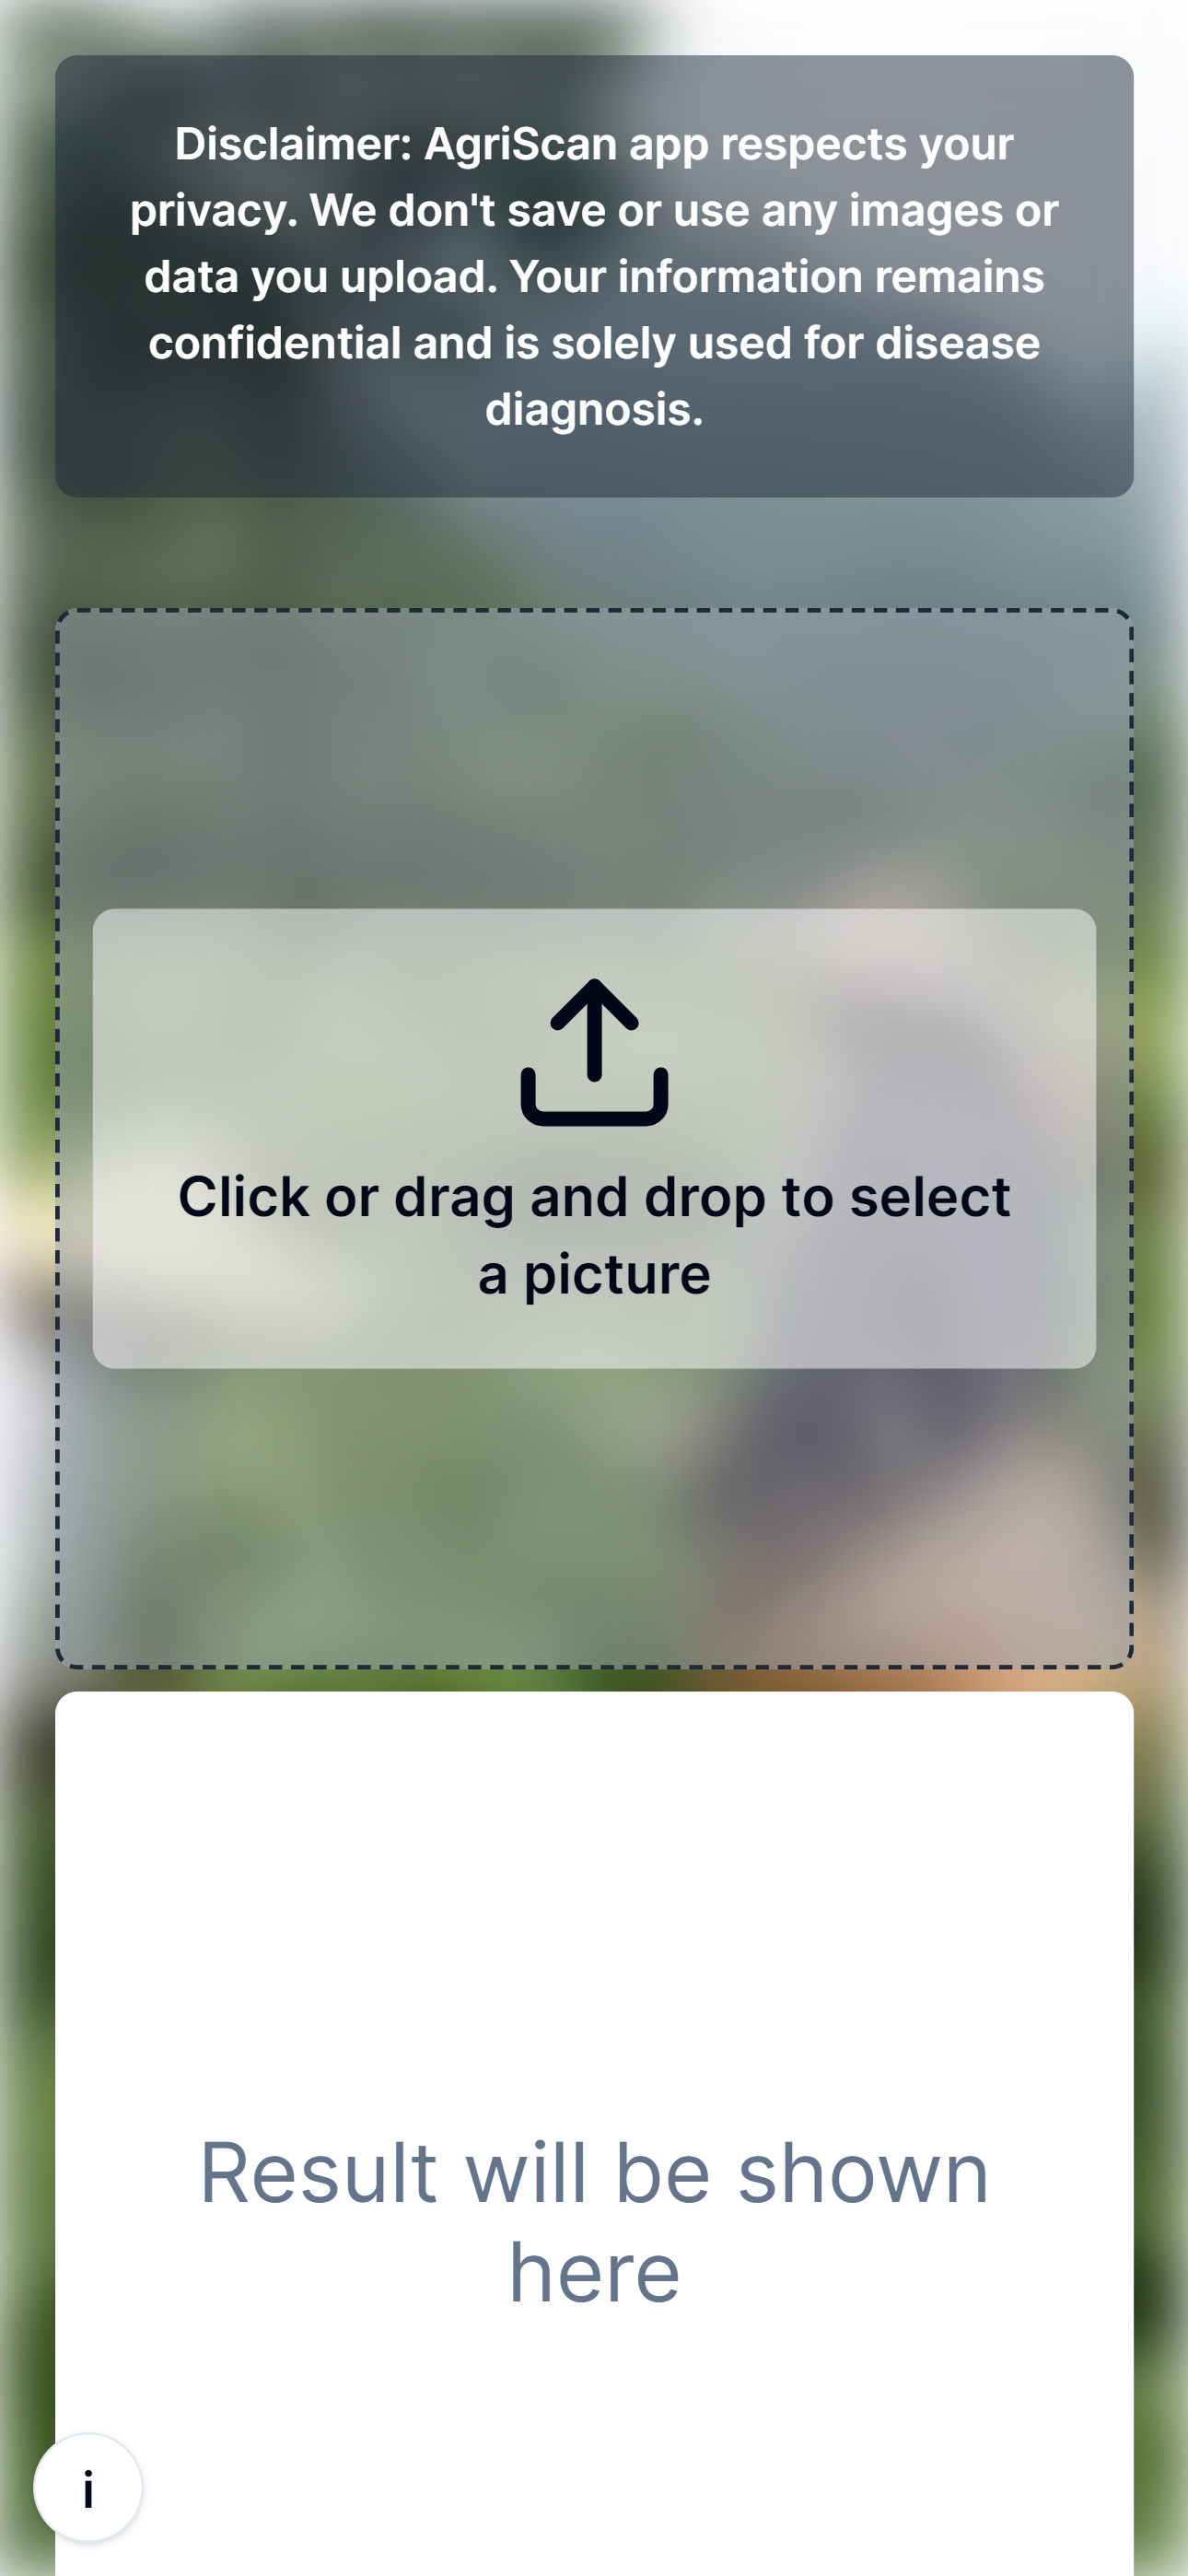
\includegraphics[height=0.4\textheight]{phone-home.png}
  \caption{Example of the plant leaf disease detection app running on mobile}
  \label{fig:mobile_version}
\end{minipage}
\hspace{0.5cm}
\begin{minipage}[b]{0.45\linewidth}
  \centering
  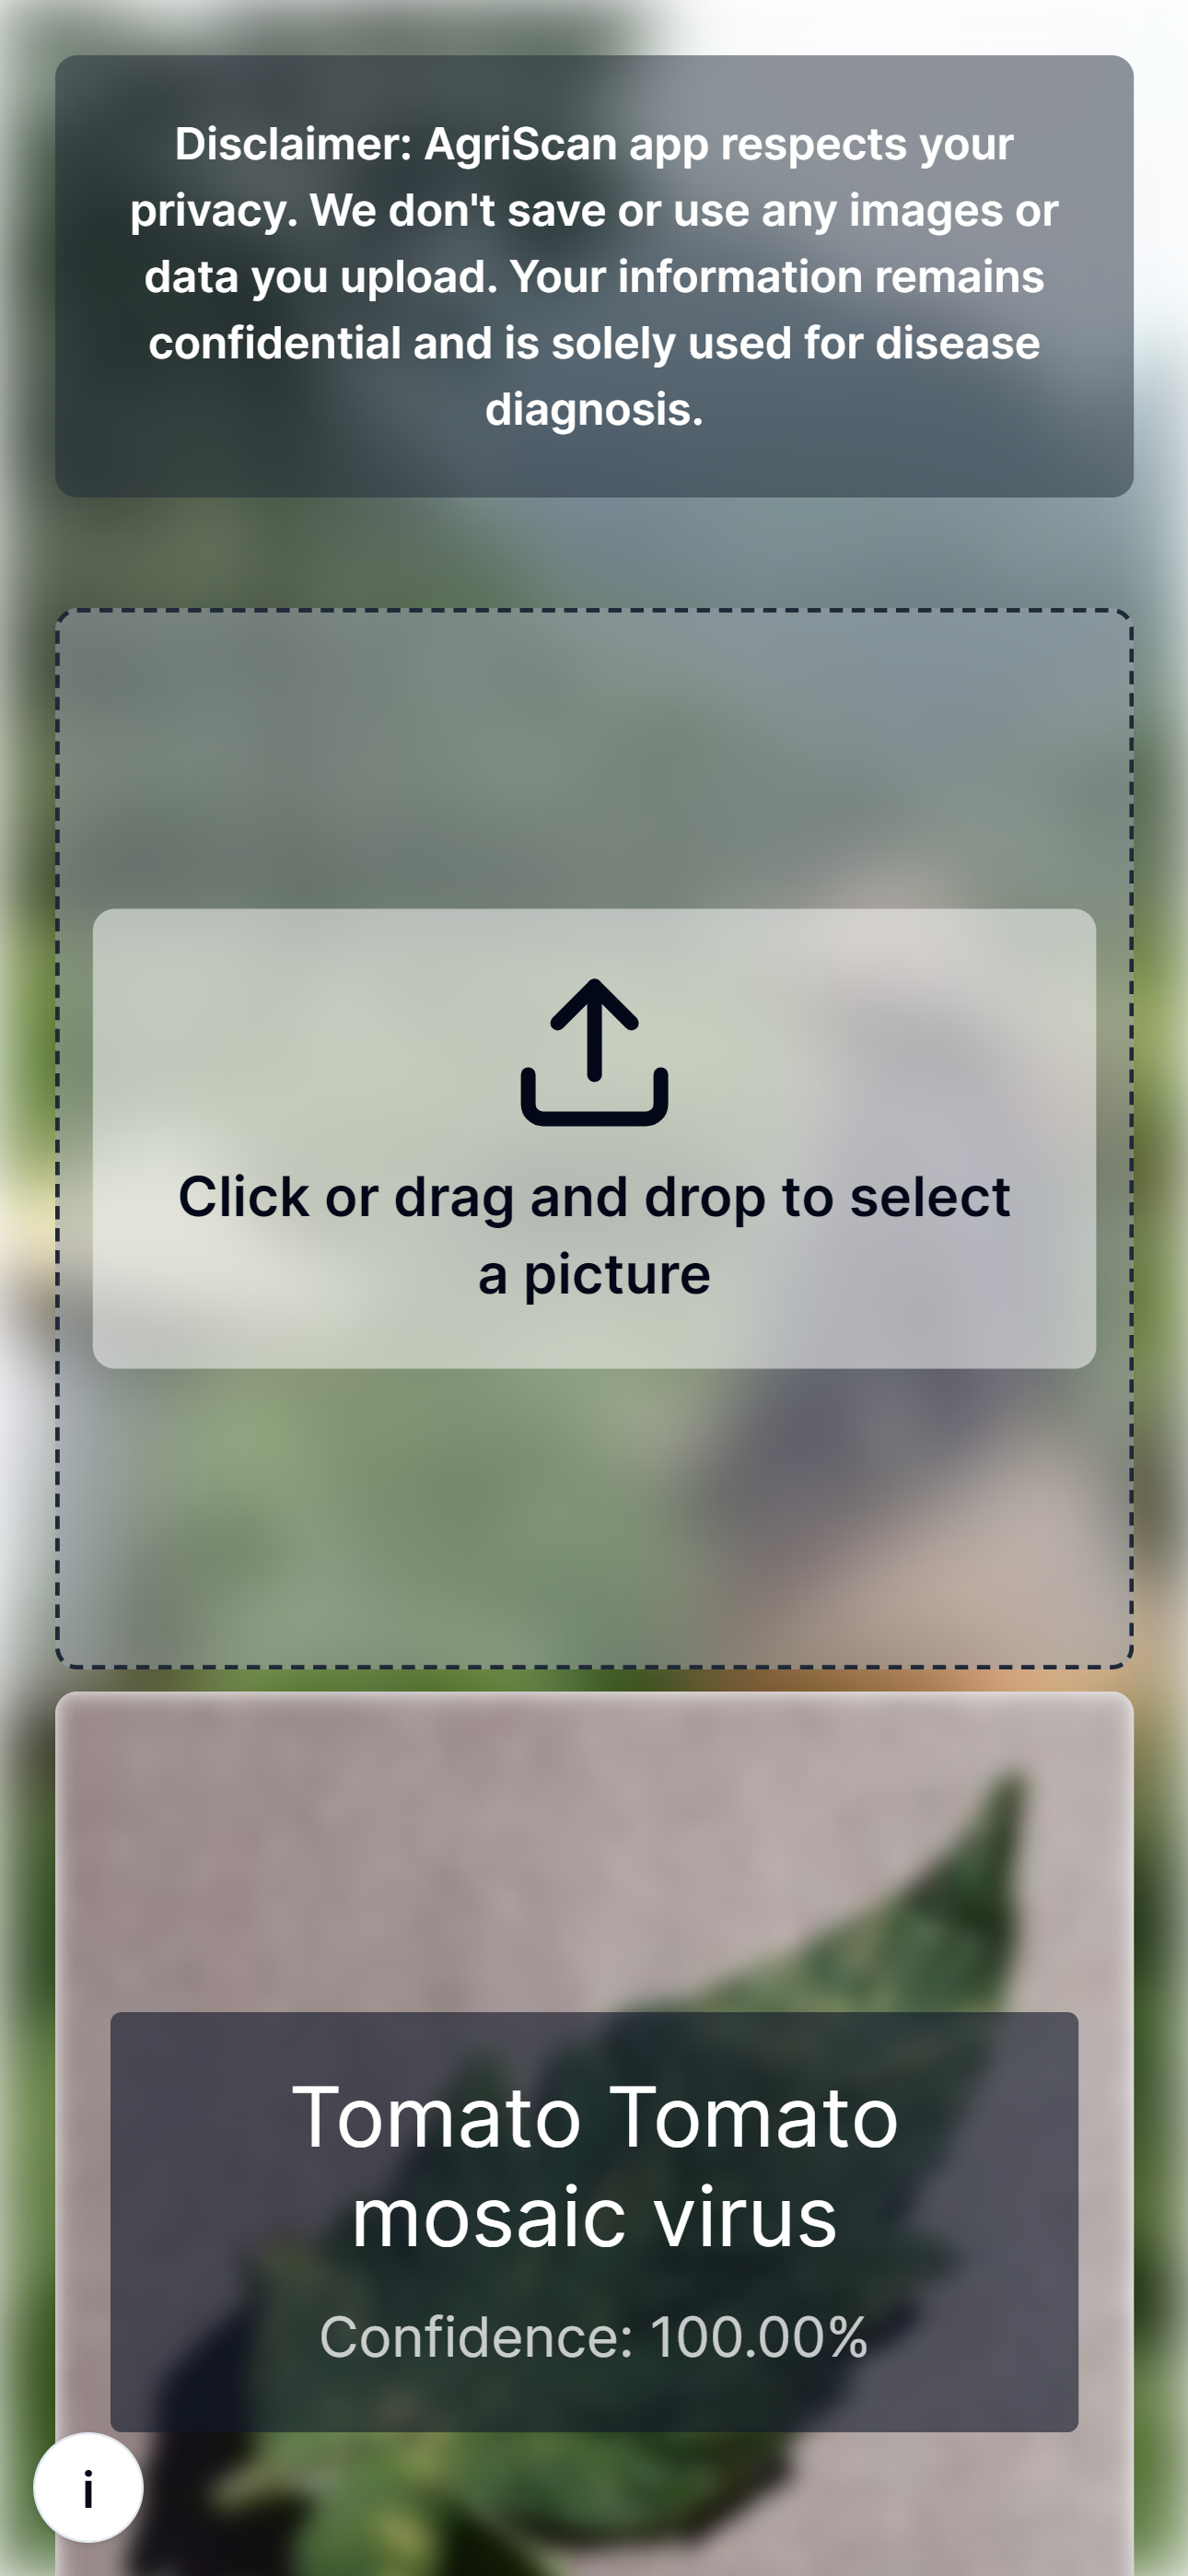
\includegraphics[height=0.4\textheight]{phone-predict.png}
  \caption{Example of the plant leaf disease detection app making a prediction}
  \label{fig:prediction_mobile}
\end{minipage}
\end{figure}

\begin{figure}[h]
  \centering
  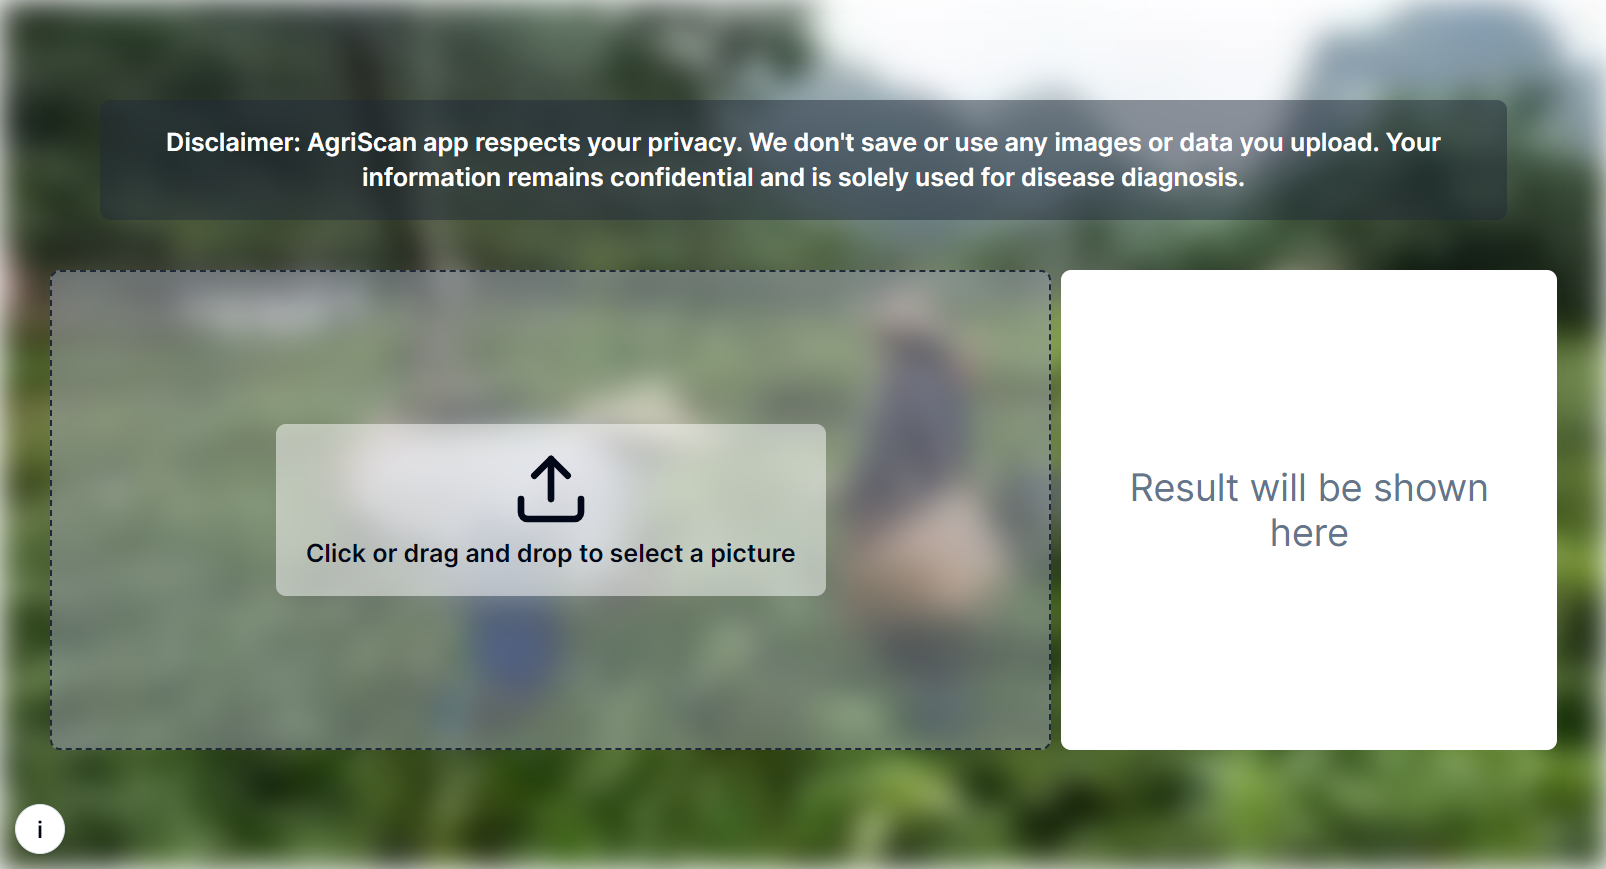
\includegraphics[width=0.5\textwidth]{pc-home.png}
  \caption{Example of the plant leaf disease detection app running on desktop}
  \label{fig:desktop_version}
\end{figure}

\begin{figure}[h]
  \centering
  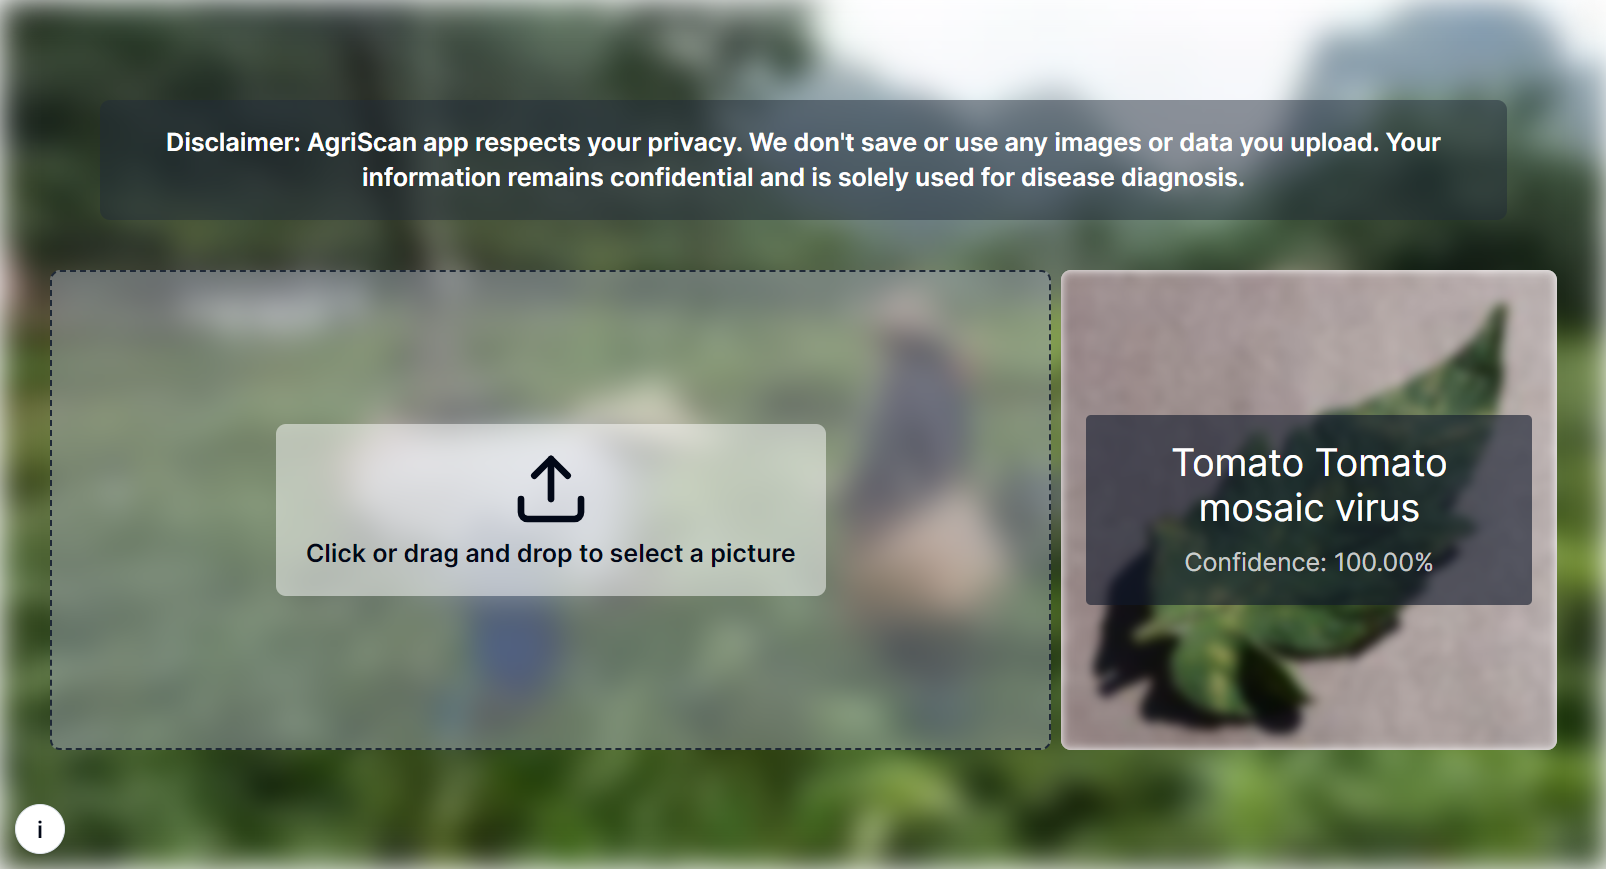
\includegraphics[width=0.5\textwidth]{pc-predict.png}
  \caption{Example of the plant leaf disease detection app making a prediction}
  \label{fig:prediction_desktop}
\end{figure}

\begin{figure}[h]
  \centering
  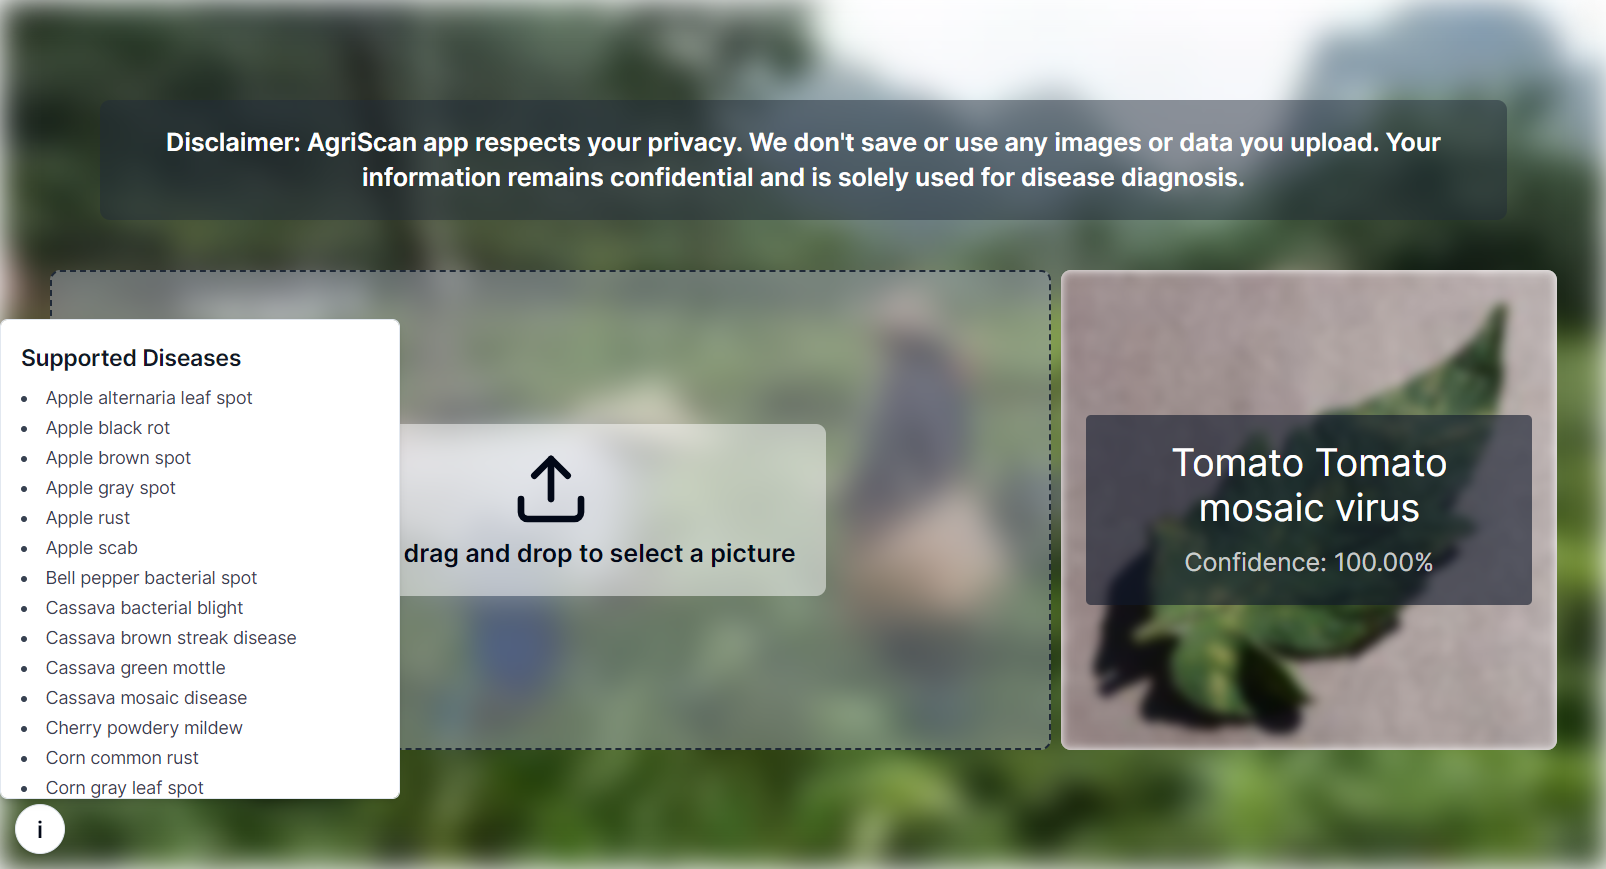
\includegraphics[width=0.5\textwidth]{pc-i-button.png}
  \caption{Example of the disclaimer button in the plant leaf disease detection app}
  \label{fig:disclaimer_button}
\end{figure}


\subsection{Deployment}

Deploying the plant leaf disease detection app involves several crucial steps to ensure accessibility and usability for users. This process encompasses various aspects, including setting up continuous integration/continuous deployment (CI/CD) pipelines, selecting appropriate cloud deployment platforms, and containerizing the application for efficient deployment and scaling.

\subsubsection{Continuous Integration/Continuous Deployment (CI/CD)}

GitHub Actions is chosen as the CI/CD solution for automating the build, testing, and deployment process of the plant leaf disease detection app for several reasons. Firstly, GitHub Actions provides seamless integration with GitHub repositories, allowing us to define workflows directly in the repository's codebase using YAML syntax. This simplifies the setup process and enables version-controlled CI/CD configurations alongside the application code.

Secondly, GitHub Actions offers a wide range of pre-built actions and workflows for common CI/CD tasks, such as running tests, building Docker images, and deploying to various cloud platforms. These actions can be easily customized and combined to create complex CI/CD pipelines tailored to the specific requirements of the app.

Additionally, GitHub Actions provides scalability and flexibility, allowing us to run workflows on GitHub-hosted virtual machines or our own self-hosted infrastructure. This ensures that we can scale our CI/CD processes according to the project's needs and integrate with external services or tools seamlessly.

In addition to that, GitHub Actions offers built-in support for triggering workflows based on events such as code pushes, pull requests, or scheduled intervals. This enables us to automate the entire development lifecycle, from code changes to deployment, without manual intervention, improving efficiency and reducing the risk of human error.


\subsubsection{Cloud Deployment (Vercel)}

Vercel is chosen as the cloud platform for deploying the frontend of the plant leaf disease detection app for several reasons. Firstly, Vercel offers seamless integration with Next.js, providing built-in support for features like serverless functions, automatic server-side rendering (SSR), and static site generation (SSG). This integration simplifies the deployment process and ensures optimal performance for Next.js applications.

Secondly, Vercel provides a global content delivery network (CDN) with edge caching, ensuring fast and reliable access to the app for users worldwide. This is essential for delivering a responsive user experience and reducing latency, especially for image-heavy applications like plant leaf disease detection.

Additionally, Vercel offers automatic scaling and zero downtime deployments, ensuring that the app can handle fluctuations in traffic and remain available even during deployment updates. This enhances the app's reliability and availability for users, minimizing disruptions to their workflow.

And Vercel provides powerful developer tools, including real-time logs, performance analytics, and environment variables management, making it easier to monitor and manage the deployed app. These tools help streamline the development and operations workflow, enabling developers to focus on building and improving the app without worrying about infrastructure management.


\subsubsection{Containerization (Docker)}

Docker is chosen as the containerization solution for the backend of the plant leaf disease detection app for several reasons. Firstly, Docker provides a lightweight and portable way to package the app and its dependencies into containers, which encapsulate the runtime environment and ensure consistency across different environments, including development, testing, and production.

Secondly, Docker containers are isolated and self-contained, allowing for easy deployment and scaling of the app across various infrastructure environments, such as on-premises servers, virtual machines, or cloud platforms. This flexibility enables seamless migration and deployment of the app without worrying about compatibility issues or dependency conflicts.

Additionally, Docker simplifies the deployment process by abstracting away the underlying infrastructure details and providing a unified interface for managing containers. With Docker Compose, we can define multi-container applications and orchestrate their deployment with a single command, streamlining the development and operations workflow.

In addition, Docker Hub provides a centralized registry for storing and sharing Docker images, allowing us to version control and distribute the app's containerized components efficiently. This enhances collaboration among team members and facilitates integration with continuous integration/continuous deployment (CI/CD) pipelines for automated testing and deployment.


\section{Final Thoughts}

\subsection{Limitations}

Despite the advancements made in developing the plant leaf disease detection app, several limitations were identified during the implementation and testing phases. One significant limitation is the accuracy of disease detection algorithms, which may vary depending on factors such as image quality, lighting conditions, and the diversity of plant species and diseases. Additionally, the app's performance may be affected by network connectivity issues, particularly during image upload and analysis processes. Furthermore, the app's usability may be hindered by limitations in device compatibility and accessibility features, which could impact the user experience for individuals with disabilities. Addressing these limitations will be crucial for enhancing the effectiveness and usability of the app in real-world scenarios.

\subsection{Future Improvements}

To address the identified limitations and further enhance the capabilities of the plant leaf disease detection app, several future improvements can be considered. Firstly, improving the accuracy of disease detection algorithms through continued research and development efforts will be paramount. This could involve collecting more diverse datasets, refining existing machine learning models, and exploring novel techniques such as transfer learning and ensemble methods. Additionally, implementing real-time feedback mechanisms and user assistance features could help improve the app's usability and accessibility. Furthermore, integrating additional features such as plant species recognition, treatment recommendations, and community-driven content sharing could enhance the app's value proposition and user engagement. Collaborating with domain experts, researchers, and end-users will be essential for identifying and prioritizing these future improvements effectively.

\section{Conclusion}

In conclusion, the development of the plant leaf disease detection app represents a significant step forward in leveraging technology to address challenges in agriculture and food security. By combining machine learning algorithms, user-friendly interfaces, and cloud-based infrastructure, the app has the potential to empower farmers and agricultural stakeholders with timely and accurate information for managing plant diseases effectively. While the app has shown promise in initial testing, there are still challenges to overcome and opportunities to explore for further improvement. By addressing limitations and prioritizing future improvements, we can continue to advance the capabilities and impact of the app, ultimately contributing to sustainable agriculture and global food security efforts.


\subsection*{References}

\begin{enumerate}
    \item Sinha, A.; Shekhawat, R.S. Review of image processing approaches for detecting plant diseases. \textit{IET Image Process.} \textbf{2020}, \textit{14}, 27–39.
    
    \item Ai, Y.; Sun, C.; Tie, J.; Cai, X. Research on recognition model of crop diseases and insect pests based on deep learning in harsh environments. \textit{IEEE Access} \textbf{2020}, \textit{8}, 686–693.
    
    \item Zeng, Q.; Ma, X.; Cheng, B.; Zhou, E.; Pang, W. Gans-based data augmentation for citrus disease severity detection using deep learning. \textit{IEEE Access} \textbf{2020}, \textit{8}, 882–891.
    
    \item Thomas, S.; Thomas, S.; Kuska, M.T.; Bohnenkamp, D.; Brugger, A.; Alisaac, E.; Wahabzada, M.; Behmann, J.; Mahlein, A.K. Benefits of hyperspectral imaging for plant disease detection and plant protection: A technical perspective. \textit{J. Plant Dis. Prot.} \textbf{2018}, \textit{125}, 5–20.
    
    \item Jiang, P.; Chen, Y.; Liu, B.; He, D.; Liang, C. Real-time detection of apple leaf diseases using deep learning approach based on improved convolutional neural networks. \textit{IEEE Access} \textbf{2019}, \textit{7}, 69–80.
    
    \item Chen, W.; Lin, Y.; Ng, F.; Liu, C.; Lin, Y. Ricetalk: Rice blast detection using internet of things and artificial intelligence technologies. \textit{IEEE Internet Things J.} \textbf{2020}, \textit{7}, 1001–1010.
    
    \item Sun, J.; Yang, Y.; He, X.; Wu, X. Northern maize leaf blight detection under complex field environment based on deep learning. \textit{IEEE Access} \textbf{2020}, \textit{8}, 79–688.
    
    \item USDA. Plant Diseases That Threaten U.S. Agriculture. 2021. Available online: \url{https://www.ars.usda.gov/crop-production-and-protection/plant-diseases/docs/npdrs/}.
    
    \item Government of Western Australia: Pests and Weeds Diseases. 2021. Available online: \url{https://www.agric.wa.gov.au/pests-weeds-diseases/diseases/}.
    
    \item Ramcharan, A.; McCloskey, P.; Baranowski, E.A.K. A mobile-based deep learning model for cassava disease diagnosis. \textit{Front. Plant Sci.} \textbf{2019}, \textit{10}, 1–8.

    \item
    Nirmalsankalana. (n.d.). Plant Diseases: Training Dataset. Kaggle. Retrieved from \url{https://www.kaggle.com/datasets/nirmalsankalana/plant-diseases-training-dataset}

    \item
    Alam, Touhidul Seyam, Chandni Barua Jowthi, and Abhijit Pathak. "Comparing pre-trained models for efficient leaf disease detection: a study on custom CNN." \textit{Journal of Electrical Systems and Information Technology} 11.1 (2024): 12.


\end{enumerate}

\end{document}
